\documentclass[11pt, oneside, fullpage, doublespace]{article}
\usepackage{geometry}                		% See geometry.pdf to learn the layout options. There are lots.
\geometry{letterpaper}                   		% ... or a4paper or a5paper or ... 
%\geometry{landscape}                		% Activate for for rotated page geometry
%\usepackage[parfill]{parskip}    		% Activate to begin paragraphs with an empty line rather than an indent
\usepackage{graphicx}				% Use pdf, png, jpg, or eps� with pdflatex; use eps in DVI mode
								% TeX will automatically convert eps --> pdf in pdflatex		
\usepackage{amssymb}

\usepackage{setspace}
\setstretch{1.5}

\title{Wireless Automobile Detection, License Plate Processing, and Data Availability Network Proposal}
\author{Kevin Emery, Santiago Gonzalez, Brandon Rodriguez, Taylor Sallee\\ \emph{Undergraduates, EECS Department, Colorado School of Mines}}
\date{March 17, 2014}




\begin{document}
\maketitle

\begin{abstract}
300 words or less. Talk about the motivation behind this project. Why it is important.
\end{abstract}

\section{Project Description}
A description

\subsection{Introduction}
Introduction. Talk about the motivation behind this project. Why it is important.

\subsection{Related Work}
\cite{stillwell2013} describes an implementation of a system to detect automobiles entering and exiting a parking lot using a magnetometer and wireless nodes based on the commercially available Arduino Fio microcontroller platform. This system uses the ubiquitous IEEE 802.15.4 communications standard to communicate automobile detection data to a central base-station based on the small, commercially available Raspberry Pi Linux computer. The project described in this proposal will augment and extend this project while collaborating closely with Stillwell, to the point of a real world deployment at the Colorado School of Mines.

\section{Proposed Work}
\subsection{Automobile Detection}
The automobile detection subsystem provides a means for detecting ingress and egress of vehicles from a parking lot. This subsystem is to be placed on the side of the road next to each parking lot entrance and exit. Automobiles will be detected using a magnetometer which perceives the induced change in the local magnetic field as the metallic structure of the vehicle passes by as described in \cite{stillwell2013}. The automobile detection subsystem will be based around the commercially available Arduino Fio 16-bit  platform which utilizes the ubiquitous Atmel ATMEGA328p microcontroller.

\begin{figure}
\begin{center}
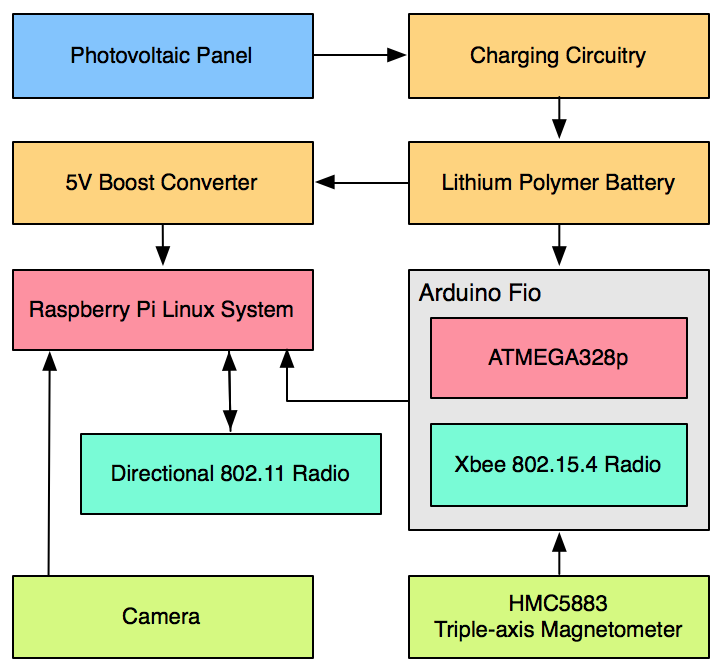
\includegraphics[width=3.5in]{autodetection}
\end{center}
\caption{Automobile Detection Subsystem Architecture}
\end{figure}

The hardware to be used for automobile detection will be contained in the same enclosure as the license plate image acquisition hardware.


The use of a magnetometer ensures that solely automobile and other large vehicles such as motorcycles are detected while pedestrians are ignored.

Work on the automobile detection subsystem will involve a variety of tests and analyses to ensure system and data integrity.


\subsection{License Plate Image Acquisition}
Kevin


\subsection{Central Basestation}
Everyone


\subsection{Server Processing}
Once an image has been determined to contain a license plate, it will be transmitted from the Acquisition Raspberry Pi to a server online via the Central Basestation Pi. The server will then be responsible for using recognition software technology to extract the digits of the license plate from the image. Upon successful completion, the textual representation of the license plate will be stored in a database residing on the server to be later integrated into a front-facing web application.

The subsystem encapsulating server processing will require a review of recognition software and literature. There exists a market for Automatic License Plate Recognition (ALPR) software that relies on Optical Character Recognition (OCR) engines to extract characters. Once an ALPR solution is chosen, it will be necessary to collect a set of test data using the Acquisition Pi to tune the workflow of character extraction. Because the system is being deployed in the metro Denver area, it can be assumed that Colorado plates will make up the majority of license plates the system will detect. Therefore, the last step will be to analyze the accuracy of the ALPR tool on extracting characters from other license plates.

\subsubsection{Review of ALPR Software}
For the scope of this project, three ALPR solutions will be evaluated to determine which is the most suitable for our purposes.

Q-Free Intrada ALPR is a license plate recognition software that offers a C++ API, as well as a cloud-based service. Both the API and cloud requests can be accomplished from a Linux server. Q-Free's software is used in countries around the world for traffic management and toll collection. The wide-ranging geography of its use mean that Intrada ALPR is likely to be reliable and accurate for all types of license plates.

OpenALPR is another C++ library for use with both North American and European plates. This library relies upon two underlying technologies: OpenCV (an open-source computer vision library) and Tesseract OCR (an OCR engine being developed and maintained by Google). The open-source nature of this project make it appealing as it can be immediately integrated without needing to obtain an educational license first.

JavaANPR markets itself as an Automated Number Plate Recognition library using Java's built-in libraries. 

\subsubsection{Collection of Test Data}

\subsubsection{Effect of Different License Plates on OCR Software}



\subsection{Web Application}
Taylor


\subsection{Deployment}
Blah


\section{Summary}
A summary \cite{johnson2012} Talk about the motivation behind this project. Why it is important.


\begin{thebibliography}{99}
\bibitem{stillwell2013} R. Stillwell, A. Wilson ``Magnetometer Parking Sensor'' \emph{EGGN 383 Final Project, Colorado School of Mines}. December 12, 2013.
\bibitem{johnson2012} X. Johnson
\end{thebibliography}





\end{document}  
